\documentclass[letterpaper,11pt]{article}
\usepackage[utf8]{inputenc}
\usepackage[spanish,mexico]{babel}
\usepackage{amsmath}
\usepackage{amsfonts}
\usepackage{amssymb}
\usepackage{graphicx}
\usepackage{caption}
\usepackage{subcaption} 
\usepackage{csquotes}

\renewcommand{\vec}[1]{\mathbf{#1}}

%%%%%%%%%%%%%%%%%%%%%%%% Control de margenes %%%%%%%%%%%%%%%%%%%%%%%%%%%%
%\setlength{\topmargin}{-1.cm}
\setlength{\oddsidemargin}{-.8cm}
\setlength{\evensidemargin}{-.8cm}
\setlength{\textheight}{24cm} 
\setlength{\textwidth}{18cm} 
\setlength{\headsep}{-2cm}


% Custom colors
\usepackage{color}
\definecolor{deepblue}{rgb}{0,0,0.5}
\definecolor{deepred}{rgb}{0.6,0,0}
\definecolor{deepgreen}{rgb}{0,0.5,0}

\usepackage{listings,xcolor}

\lstset{language=Mathematica}
\lstset{basicstyle={\sffamily\footnotesize},
  numbers=left,
  numberstyle=\tiny\color{gray},
  numbersep=5pt,
  breaklines=true,
  captionpos={t},
  frame={lines},
  rulecolor=\color{black},
  framerule=0.5pt,
  columns=flexible,
  tabsize=2
}

\author{Carlos Manuel Rodríguez Martínez}
\title{Análisis de patrones en autómata celular Wolfram regla 30}
\begin{document}
\maketitle

\section{Análisis de la fila central del autómata celular regla 30}
El autómata celular elemental de regla 30 se construye a partir de las reglas que se muestran en la figura \ref{fig:reglas}. Al utilizar una condición inicial con un recuadro del mapa con valor $1$ y evolucionar el sistema se obtiene un mapa como el que se muestra en la figura \ref{fig:automata}.

\begin{figure}[h!]
\centering
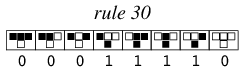
\includegraphics[scale=0.6]{img/Reglas}
\caption{Reglas para construir el autómata celular 30. \cite{MathWorld}}
\label{fig:reglas}
\end{figure}

\begin{figure}[h!]
\centering
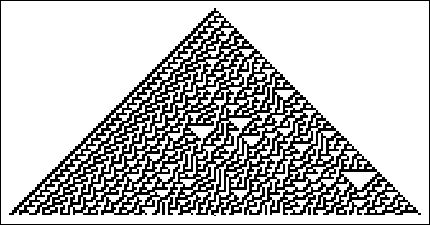
\includegraphics[scale=0.5]{img/Figura1}
\caption{Autómata celular.}
\label{fig:automata}
\end{figure}

La regla 30 del autómata celular elemental tiene la propiedad de que la aparición de ceros y unos es totalmente aleatoria, lo cual lo hace un buen generador de números aleatorios. Se analizó la frecuencia de aparición de unos y ceros en la fila central.

\begin{figure}[h!]
\begin{subfigure}{.5\textwidth}
	\centering
	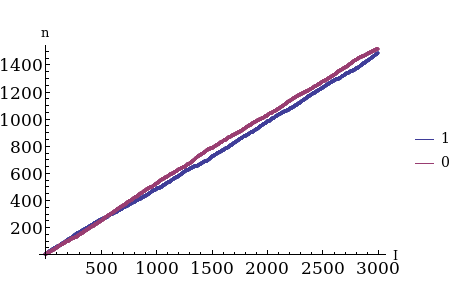
\includegraphics[scale=0.55]{img/AC_Grupo1}
	\caption{Frecuencia de $0$ y $1$.}
\end{subfigure}%
\begin{subfigure}{.5\textwidth}
	\centering
	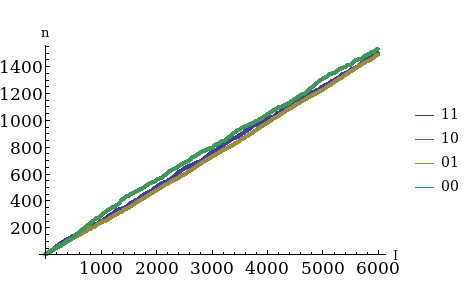
\includegraphics[scale=0.55]{img/AC_Grupo2}
	\caption{Frecuencia de $00$, $01$, $10$, $11$.}
\end{subfigure}%
\caption{Frecuencia de aparición de patrones respecto a iteraciones en AC.}
\label{fig:acpat1}
\end{figure}
\begin{figure}[h!]
\begin{subfigure}{.5\textwidth}
	\centering
	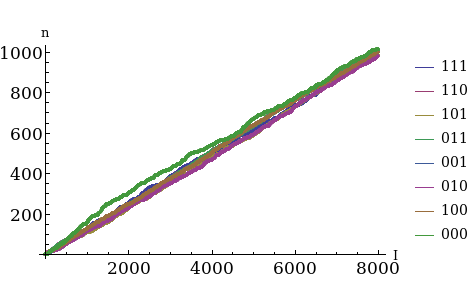
\includegraphics[scale=0.55]{img/AC_Grupo3}
	\caption{Frecuencia de patrones de 3 dígitos.}
\end{subfigure}%
\caption{Frecuencia de aparición de patrones respecto a iteraciones en AC.}
\label{fig:acpat2}
\end{figure}

\clearpage

El código utilizado para generar las gráficas es el siguiente.
\begin{lstlisting}[language=Mathematica,caption={Código para patrones de dos dígitos}]
CountPattern[list_, pat_] := Count[Partition[list, Length[pat], 1], pat]
lista11 = {};
lista10 = {};
lista01 = {};
lista00 = {};
maxiter = 6000;
ac = CellularAutomaton[30, {{1}, 0}, maxiter ];
aclist = ac[[All, Ceiling[Length[ac[[1]]]/2]]];
Do[
 list = aclist[[1 ;; iter]];
 v11 = CountPattern[list, {1, 1}];
 v10 = CountPattern[list, {1, 0}];
 v01 = CountPattern[list, {0, 1}];
 v00 = CountPattern[list, {0, 0}];
 AppendTo[lista11, v11];
 AppendTo[lista10, v10];
 AppendTo[lista01, v01];
 AppendTo[lista00, v00];
 , {iter, 1, maxiter}
 ]
ListPlot[{lista11, lista10, lista01, lista00}, 
 PlotLegends -> LineLegend[{"11", "10", "01", "00"}], 
 AxesLabel -> {Style["I", 12], Style["n", 12]}, 
 BaseStyle -> {FontSize -> Scaled[.045]}, ImageSize -> {400, 300}]
\end{lstlisting}

\section{Comparación con generador de números aleatorios}

Se realizó una comparación con el algoritmo de generación de números aleatorios conocido como \textit{Mersenne-Twister}. Este algoritmo es uno de los más usados por su velocidad y alto periodo de frecuencia ($2^{19937}-1$). No se encontraron diferencias significativas al hacer el conteo de la frecuencia de aparición de patrones en el \textit{Mersenne-Twister} respecto al autómata celular.

\begin{figure}[h!]
\begin{subfigure}{.5\textwidth}
	\centering
	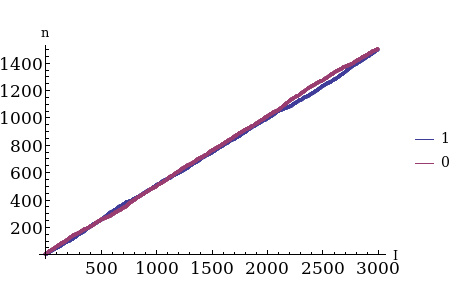
\includegraphics[scale=0.55]{img/Mersenne_Grupo1}
	\caption{Frecuencia de $0$ y $1$.}
\end{subfigure}%
\begin{subfigure}{.5\textwidth}
	\centering
	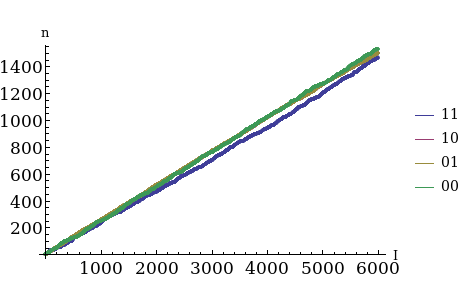
\includegraphics[scale=0.55]{img/Mersenne_Grupo2}
	\caption{Frecuencia de $00$, $01$, $10$, $11$.}
\end{subfigure}%
\caption{Frecuencia de aparición de patrones respecto a iteraciones en MT.}
\label{fig:acpat1}
\end{figure}
\begin{figure}[h!]
\begin{subfigure}{.5\textwidth}
	\centering
	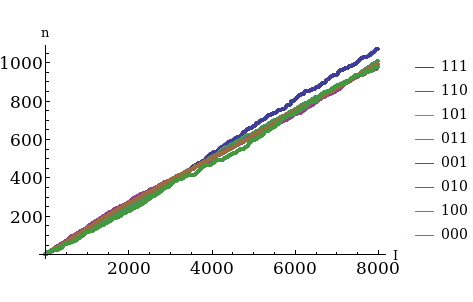
\includegraphics[scale=0.55]{img/Mersenne_Grupo3}
	\caption{Frecuencia de patrones de 3 dígitos.}
\end{subfigure}%
\caption{Frecuencia de aparición de patrones respecto a iteraciones en MT.}
\label{fig:acpat2}
\end{figure}


\section{Referencias}
\renewcommand*{\refname}{}
\begin{thebibliography}{100}
\bibitem{MathWorld} Weisstein, Eric W. \enquote{Elementary Cellular Automaton.} From MathWorld--A Wolfram Web Resource. http://mathworld.wolfram.com/ElementaryCellularAutomaton.html

\end{thebibliography}

\end{document}